\documentclass[border=5mm]{standalone}
\usepackage[utf8]{inputenc}
\usepackage[T1]{fontenc}
\usepackage{amsmath}
\usepackage{tikz}
\usepackage{pgfplots}
\pgfplotsset{compat=1.18}
\usetikzlibrary{arrows.meta}
\definecolor{utnblue}{RGB}{0, 51, 102}

% Ej6b: x(t)=(t+1)u(t), h(t)=e^{-2t}u(t)
% y(t) = (1/4)(2t + 1 - e^{-2t}) u(t)
% Layout: fila superior x | h (escalas distintas), abajo y (ancho completo).

\begin{document}
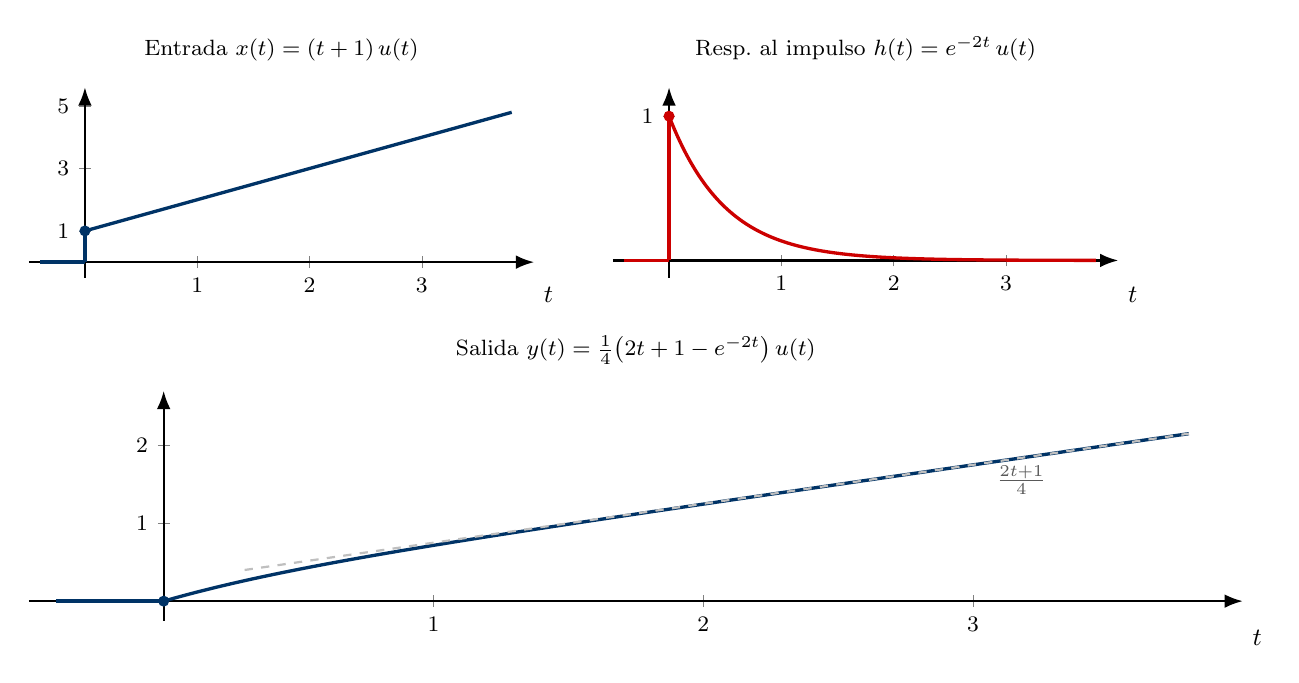
\begin{tikzpicture}[>=Latex, font=\small]

\colorlet{xcol}{utnblue}
\colorlet{hcol}{red!80!black}

% =====================================================================
% PANEL x(t)
% =====================================================================
\begin{axis}[
    name=panX,
    width=8cm, height=4cm,
    axis lines=center,
    xlabel={$t$},
    xlabel style={anchor=north west, at={(axis description cs:1,0)}},
    xmin=-0.5, xmax=4,
    ymin=-0.5, ymax=5.6,
    clip=false,
    axis line style={->, thick},
    xtick={0,1,2,3},
    ytick={0,1,3,5},
    every tick label/.style={font=\footnotesize},
    title={\footnotesize Entrada $x(t) = (t+1)\,u(t)$},
]
    \addplot[xcol, very thick, domain=-0.4:0, samples=2] {0};
    \addplot[xcol, very thick, domain=0:3.8, samples=2] {x+1};
    \draw[xcol, very thick] (axis cs:0,0) -- (axis cs:0,1);
    \fill[xcol] (axis cs:0,1) circle (2pt);
\end{axis}

% =====================================================================
% PANEL h(t)
% =====================================================================
\begin{axis}[
    name=panH,
    at={(panX.east)}, anchor=west, xshift=1cm,
    width=8cm, height=4cm,
    axis lines=center,
    xlabel={$t$},
    xlabel style={anchor=north west, at={(axis description cs:1,0)}},
    xmin=-0.5, xmax=4,
    ymin=-0.12, ymax=1.2,
    clip=false,
    axis line style={->, thick},
    xtick={0,1,2,3},
    ytick={0,1},
    every tick label/.style={font=\footnotesize},
    title={\footnotesize Resp.\ al impulso $h(t) = e^{-2t}\,u(t)$},
]
    \addplot[hcol, very thick, domain=-0.4:0, samples=2] {0};
    \addplot[hcol, very thick, domain=0:3.8, samples=200] {exp(-2*x)};
    \draw[hcol, very thick] (axis cs:0,0) -- (axis cs:0,1);
    \fill[hcol] (axis cs:0,1) circle (2pt);
\end{axis}

% =====================================================================
% PANEL y(t) (ancho completo)
% =====================================================================
\begin{axis}[
    name=panY,
    at={(panX.below south west)}, anchor=north west, yshift=-1cm,
    width=17cm, height=4.5cm,
    axis lines=center,
    xlabel={$t$},
    xlabel style={anchor=north west, at={(axis description cs:1,0)}},
    xmin=-0.5, xmax=4,
    ymin=-0.25, ymax=2.7,
    clip=false,
    axis line style={->, thick},
    xtick={0,1,2,3},
    ytick={0,1,2},
    every tick label/.style={font=\footnotesize},
    title={\footnotesize Salida $y(t) = \tfrac{1}{4}\bigl(2t+1-e^{-2t}\bigr)\,u(t)$},
]
    \addplot[utnblue, very thick, domain=-0.4:0, samples=2] {0};
    \addplot[utnblue, very thick, domain=0:3.8, samples=200] {(2*x + 1 - exp(-2*x))/4};
    \fill[utnblue] (axis cs:0, 0) circle (2pt);

    % asíntota lineal
    \addplot[domain=0.3:3.8, dashed, thick, gray!50] {(2*x+1)/4};
    \node[font=\footnotesize, gray!70!black, anchor=west]
        at (axis cs:3.05, 1.55) {$\tfrac{2t+1}{4}$};
\end{axis}

\end{tikzpicture}
\end{document}
